We used a subset of the participants present in \citet{Martinez2019-mm} and \citet{Bouffard2019-fd}, as well as the same experimental procedures and data collection summarized below.

\subsection{Participants}\label{subsec:participants}

Forty healthy participants, including 20 women ($21.4 \pm 1.9$ years; $167.7 \pm 7.1$~cm; $61 \pm 8.9$~kg) and 20 men ($24.9 \pm 3.2$ years; $179.3 \pm 7.9$~cm; $75.1 \pm 12.1$~kg) took parts in this study.
Participants could safely perform physical activity, were free from self-reported musculoskeletal disorders and none reported significant disability related to their upper extremity or their back (see further details in \citet{Martinez2019-mm} and \citet{Bouffard2019-fd}).
Participants were fully advised of the experimental content and each of them provided written informed consent.
The research protocol was approved by the University of Montreal Ethics Committee (No. 15--016-CERES-P).

\subsection{Experimental procedures}\label{subsec:experimental-procedures}

After a static trial, participants moved an instrumented box of 6 and 12~kg between two shelves.
Shelf heights were adjusted at the hip and eye levels of each participant (Figure 1).
We set the box mass at 6 and 12~kg, which corresponds to the maximum acceptable mass in our configuration~\cite{Snook1991-yo}.
Three lifts were performed for each mass in random order with 30 s rest periods in-between, with additional recovery time when needed.
The movement was split into three phases: the pulling (1-20\% of the trial), lifting (21-60\%) and dropping (61-100\%) phases (Figure~\ref{fig:phases}).

\begin{figure}[H]
    \centering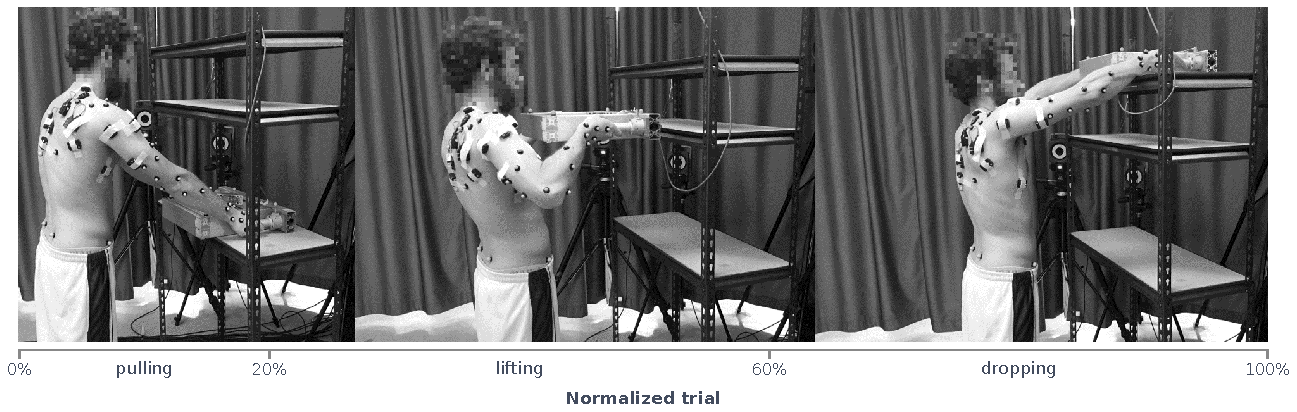
\includegraphics[width=1\linewidth]{fig/phases.pdf}
    \caption{The pulling (from 0 to 20\% of the trial), lifting (21-60\%) and dropping (61-100\%) phases of the lifting task.}
    \label{fig:phases}
\end{figure}

\subsection{Data collection}\label{subsec:data-collection}

The right handle of the box was instrumented with a 6-degree-of-freedom force sensor (Sensix, Poitiers, France) used to measure external forces and define the beginning and the end of each trial.
Markers kinematics were recorded with a VICON™ motion analysis system (Oxford Metrics Ltd, Oxford, UK) and the \citet{Jackson2012-uj} markers model.
Assuming that the left and right sides of the upper body behaved symmetrically during a symmetrical lifting task~\cite{Bouffard2019-fd, Martinez2019-mm, Nielsen1998-fc}, only the right side of the participant was evaluated.

\subsection{Data processing}\label{subsec:data-processing}

All musculoskeletal computations were carried using the OpenSim software API~\cite{Delp2007-ol} and batch processed with the Pyomeca and Pyosim Python libraries~\cite{martinez-pyo}.
The generalized coordinates were computed by inverse kinematics from a custom scaled \citet{Wu2016-kw} upper extremity model (details in~\ref{sec:custom-wu-shoulder-model}).
Then, muscle activations and forces were estimated by static optimization from the generalized coordinates and external forces measured with the instrumented box~\cite{Anderson2001-ma, Erdemir2007-ou}.
These muscle forces were resolved by minimizing the sum of squared muscle activations.
Residual actuators, that account for the non-modelled passive structures~\cite{Hicks2015-wl}, have been added for all joints.
Finally, the glenohumeral joint reaction forces were calculated.
These forces correspond to the internal loads applied on the joint.
The glenohumeral forces were expressed in the local reference frame of the glenoid.
From these forces, we reported the relative time spent beyond a shear-compression dislocation ratio ($\frac{\textrm{shear}}{\textrm{compression}} > 56$\%~\cite{Dickerson2007-qj}).
Three \textsc{ulmd} risk indicators were extracted from this data processing: (1) the sum of muscle activations, (2) the sum of muscle forces and (3) the relative time spent beyond a shear-compression dislocation ratio.

\subsection{Statistics}\label{subsec:statistics}

Time series risk indicators (sum of muscle activations and forces) were time normalized to 1000 data points.
Women and men were then compared using the statistical parametric mapping procedure implemented in the spm1d Python library~\cite{Pataky2010-zh}.
This technique avoids the information loss associated with standard methods which reduce time series into a single, arbitrary, data point (such as mean or median) while controlling for type $\alpha$ error due to multiple comparisons.
Nonparametric testing~\cite{Nichols2002-ri} was chosen as it leads to results qualitatively identical to parametric testing, while being robust to non-normal and non-spherical data~\cite{Pataky2015-ss}.
We tested the main and interaction effects between sex (women \textit{vs} men) and mass (6~kg \textit{vs} 12~kg) on the three \textsc{ulmd} risk indicators with a nonparametric two-way \textsc{anova}.
Each significant difference was reported with the cluster duration, the mean difference, the p-value and the \citet{Cohen2013-tj} $d$ effect size (\textsc{es}).
\textsc{es} was interpreted as large (\textsc{es} $\geq$ 0.8), medium (0.8 $>$ \textsc{es} $\geq$ 0.5) or small (\textsc{es} $<$ 0.5).
While the analyses described above make it possible to analyze time series, statistical inferences were also carried on empirical cumulative distribution functions (\textsc{ecdf}).
The \textsc{ecdf} evaluated at $x$ is defined as the fraction of the points of data which are $\leq x$.
Thus, the \textsc{ecdf} can be graphically represented as the percentile ($x$-axis) associated with each value ($y$-axis).
This method allows exploring distribution objectively, without choosing any parameters as opposed to other techniques (number of binning classes for histograms or bandwidth for kernel density estimation).